\documentclass{article}
\usepackage{amsmath,amsthm}
\usepackage{amssymb,latexsym}
\usepackage{epsfig}
\usepackage{hyperref}
\usepackage{float}
\usepackage{fullpage}
\usepackage{enumerate}
\usepackage{paralist}
\usepackage{times}
\usepackage{tikz}
\usetikzlibrary{automata,positioning}


\newtheorem{theorem}{Theorem}
\newtheorem{corollary}[theorem]{Corollary}
\newtheorem{question}[theorem]{Question}
\newtheorem{lemma}[theorem]{Lemma}
\newtheorem{observation}[theorem]{Observation}
\newtheorem{proposition}{Proposition}
\newtheorem{definition}[theorem]{Definition}
\newtheorem{claim}[theorem]{Claim}
\newtheorem{fact}[theorem]{Fact}
\newtheorem{assumption}[theorem]{Assumption}
\newtheorem{example}{Example}
\newtheorem{conjecture}[theorem]{Conjecture}
\newtheorem{alg}[theorem]{Algorithm}

\newcommand{\myparagraph}[1]{\paragraph{#1.}}

\newcommand{\set}[1]{{\left\{#1\right\}}}    % braces for set notation
\newcommand{\ve}[1]{\mathbf{#1}}
\newcommand{\abs}[1]{\left\lvert #1 \right\rvert}

\newcommand{\complex}{{\mathbb C}}
\newcommand{\reals}{{\mathbb R}}
\newcommand{\ints}{{\mathbb Z}}
\newcommand{\nats}{{\mathbb N}}

\newcommand{\enc}[1]{\left<#1\right>}

\newcommand{\spa}[1]{\mathcal{#1}}

\mathchardef\mhyphen="2D

\bibliographystyle{alpha}

\begin{document}

\title{CMSC303 Introduction to Theory of Computation, VCU\\Spring 2017, Assignment 2\\Matthew Bowers}
\date{}
\maketitle

Total marks: $29$ marks $+$ $5$ bonus marks $+$ $3$ bonus marks for LaTeX\\

Unless otherwise noted, the alphabet for all questions below is assumed to be $\Sigma=\set{0,1}$.

\begin{enumerate}
    \item (6 marks) This question tests your comfort with ``boundary cases'' of DFA's. Draw the state diagrams of DFA's recognizing each of the following languages.
    \begin{enumerate}
        \item (2 marks) $L=\set{\epsilon}$ for $\epsilon$ the empty string.

	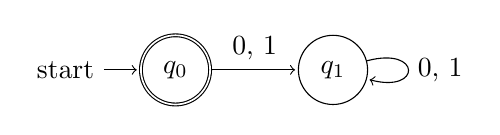
\begin{tikzpicture}[shorten >=1pt,node distance=2cm,on grid,auto] 
		\node[state,initial, accepting] (q_0)   {$q_0$}; 
		\node[state] (q_1) [right=of q_0] {$q_1$};
		\path[->]
			(q_0) edge  node {0, 1} (q_1)
			(q_1) edge [loop right] node {0, 1} ();
   	\end{tikzpicture}
        \item (2 marks) $L=\emptyset$.\\
	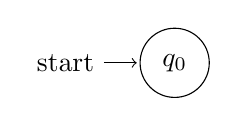
\begin{tikzpicture}[shorten >=1pt,node distance=2cm,on grid,auto]
		\node[state, initial] (q_0) {$q_0$};
	\end{tikzpicture}
        \item (2 marks) $L = \set{0,1}^*$.\\
	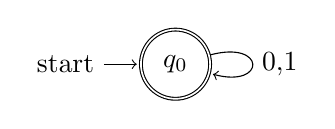
\begin{tikzpicture}[shorten >=1pt,node distance=2cm,on grid,auto]
		\node[state, initial, accepting] (q_0) {$q_0$};
		\path[->]
			(q_0) edge [loop right] node {0,1} ();
	\end{tikzpicture}
    \end{enumerate}
    \item (8 marks) This question tests your ability to design DFAs and NFAs.
        \begin{enumerate}
        \item (2 marks) Draw the state diagram for a DFA recognizing language $L_1 = \set{x\mid x \text{ contains at least two 1s}}$.\\
		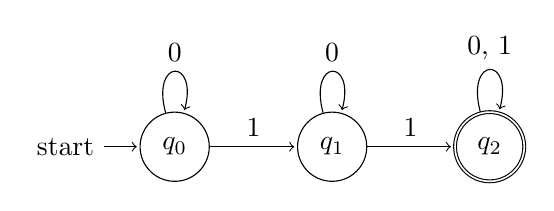
\begin{tikzpicture}[shorten >=1pt,node distance=2cm,on grid,auto] 
			\node[state,initial] (q_0)   {$q_0$}; 
			\node[state] (q_1) [right=of q_0] {$q_1$};
			\node[state, accepting] (q_2) [right=of q_1] {$q_2$};
			\path[->]
				(q_0) edge  node {1} (q_1)
				(q_0) edge [loop above] node {0} ()
				(q_1) edge  node {1} (q_2)
				(q_1) edge [loop above] node {0} ()
				(q_2) edge [loop above] node {0, 1} ();
   		\end{tikzpicture}
        \item (2 marks) Draw the state diagram for a DFA recognizing language $L_2 = \set{x\mid x \text{ contains at most one 0}}$.\\
		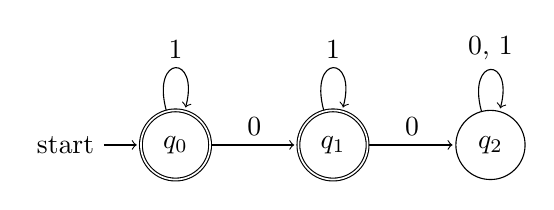
\begin{tikzpicture}[shorten >=1pt,node distance=2cm,on grid,auto] 
			\node[state,initial, accepting] (q_0)   {$q_0$}; 
			\node[state, accepting] (q_1) [right=of q_0] {$q_1$};
			\node[state] (q_2) [right=of q_1] {$q_2$};
			\path[->]
				(q_0) edge  node {0} (q_1)
				(q_0) edge [loop above] node {1} ()
				(q_1) edge  node {0} (q_2)
				(q_1) edge [loop above] node {1} ()
				(q_2) edge [loop above] node {0, 1} ();
   		\end{tikzpicture}
	\newpage
        \item (4 marks) Draw the state diagram for a NFA recognizing language $L_3=L_1\cup L_2$.\\
		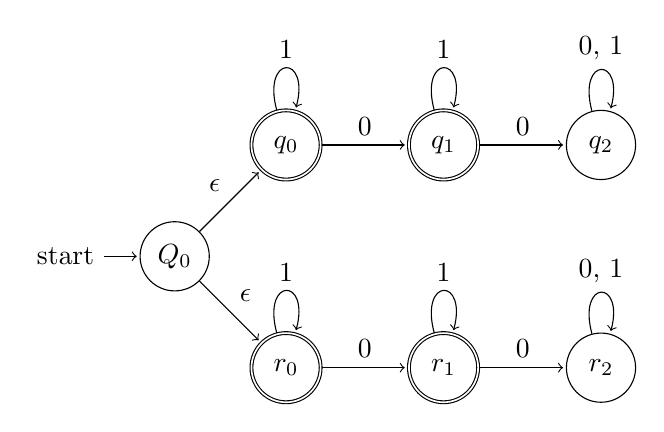
\begin{tikzpicture}[shorten >=1pt,node distance=2cm,on grid,auto] 
			\node[state, initial] (Q_0) {$Q_0$};
			\node[state, accepting] [above right=of Q_0] (q_0)   {$q_0$}; 
			\node[state, accepting] (q_1) [right=of q_0] {$q_1$};
			\node[state] (q_2) [right=of q_1] {$q_2$};
			\node[state, accepting] (r_0) [below right=of Q_0] {$r_0$}; 
			\node[state, accepting] (r_1) [right=of r_0] {$r_1$};
			\node[state] (r_2) [right=of r_1] {$r_2$};
			\path[->]
				(Q_0) edge node {$\epsilon$} (q_0)
				(Q_0) edge node {$\epsilon$} (r_0)
				(r_0) edge  node {0} (r_1)
				(r_0) edge [loop above] node {1} ()
				(r_1) edge  node {0} (r_2)
				(r_1) edge [loop above] node {1} ()
				(r_2) edge [loop above] node {0, 1} ()
				(q_0) edge  node {0} (q_1)
				(q_0) edge [loop above] node {1} ()
				(q_1) edge  node {0} (q_2)
				(q_1) edge [loop above] node {1} ()
				(q_2) edge [loop above] node {0, 1} ();
   		\end{tikzpicture}
        \end{enumerate}
    \item (3 marks) In this question, you will study closure of regular languages under certain operations. Specifically, show that if $M$ is a DFA that recognizes language $B$, then swapping the accept and nonaccept states in $M$ yields a new DFA $M'$ recognizing the complement of $B$, $\overline{B}$. Which operation does this imply the regular languages are closed under?\\
\\
\begin{proof} Let the DFA $M$ := {Q, $\Sigma$, $\delta$, $q_0$, $F$}\\
Define a new FDA $M'$ :=  {Q, $\Sigma$, $\delta$, $q_0$, $Q-F$}\\
By changing the accept states to the compliment we ensure that any string which was accepted by the first machine will be rejected by the second and any string rejected by the first machine will be accepted by the first. We can thus conclude that regular languages are closed under compliment because we can construct a DFA which can recognize the compliment of any regular language.
\end{proof}
    \item (6 marks) This question tests your ability to prove a language is regular using the closure properties of regular languages. Given languages $A$ and $B$, define the operation $\cdot$ as \[A \cdot B :=\set{x\mid x\in A \text{ and } x \text{ does not contain any string in }B\text{ as a substring.}}.\] Prove that the class of regular languages is closed under the $\cdot$ operation. (Hint: Recall that by DeMorgan's law, for any sets $X$ and $Y$, one has $X\cap Y=\neg(\neg X \cup \neg Y)$.)\\
\begin{proof}
The language can be written as a regular expression $A\cap \overline{(\Sigma^*B\Sigma^*)}$\\
By DeMorgan's Law this can be rewritten $\overline{(\overline{A} \cup (\Sigma^*B\Sigma^*)}$\\
It has already been shown that regular languages are closed under concatination, star, union, and negation so this is a regular language meaning that regular languages are closed under $\cdot$.
\end{proof}
    \item (6 marks) This question tests your understanding of the equivalence between DFAs and NFAs. Consider NFA $M = (\set{q_1,q_2}, \set{0,1},\delta, q_1, \set{q_1})$ for $\delta$ defined as:
        \[
\begin{tabular}{|c|c|c|c|}
  \hline
  $\delta$ & 0 & 1 &$\epsilon$  \\
  \hline
  $q_1$ & $\set{q_1,q_2}$ & $\set{q_2}$ &$\emptyset$\\
  $q_2$ & $\emptyset$ & $\set{q_1}$& $\set{q_1}$\\
  \hline
\end{tabular}
        \]
 Draw both the state diagrams for $M$ and for a DFA $M'$ equivalent to $M$ based on the construction of Theorem 1.39 in the text (recall the latter proves that DFAs and NFAs are equivalent).\\
	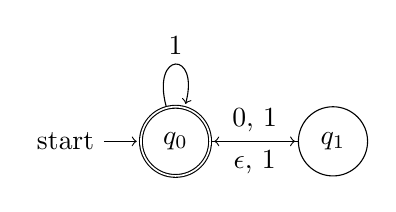
\begin{tikzpicture}[shorten >=1pt,node distance=2cm,on grid,auto] 
		\node[state,initial, accepting] (q_0)   {$q_0$}; 
		\node[state] (q_1) [right=of q_0] {$q_1$};
		\path[->]
			(q_0) edge  node {0, 1} (q_1)
			(q_0) edge [loop above] node {1} ()
			(q_1) edge node {$\epsilon$, 1} (q_0);
   	\end{tikzpicture}\\
	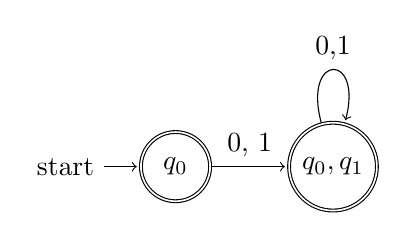
\begin{tikzpicture}[shorten >=1pt,node distance=2cm,on grid,auto] 
		\node[state, initial, accepting] (q_0) {$q_0$};
		\node[state, accepting] [right=of q_0] (q_01) {$q_0, q_1$};
		\path[->]
			(q_0) edge node {0, 1} (q_01)
			(q_01) edge [loop above] node {0,1} ();
	\end{tikzpicture}
    \item (Bonus, 5 marks) This question demonstrates that although DFAs and NFAs are equivalent in terms of the sets of languages they recognize, they are \emph{provably not} equivalent in terms of efficiency (i.e. DFAs may require \textbf{many} more states to recognize a language than an NFA). Consider the language $C_k=\Sigma^* 0 \Sigma^{k-1}$ for $k\geq 1$. Convince yourself that an NFA with $k+1$ states for recognizing $C_k$ exists (no need to include this in your assignment answer). Now, prove that for any $k$, $C_k$ cannot be recognized by a DFA with less than $2^k$ states.\\
\textbf{Part 1}
\begin{proof} An NFA to recognize such a language would have as a submachine a DFA which recognizes $0\Sigma^k-1$ this will require exactly k states. One to accept the 0 then k - 1 to read in the remaining characters. To get the NFA you would add a single state which loops on itself given any input. The nature of these transitions means that the DFA would always have to be in a state which includes $q_0$ from the initial machine. Since we know that a DFA can be formed by using $P(Q)$ of the states of the original NFA we begin with that power set and remove every state which does not include $q_0$. The original power set has $2^k+1$ sets. We form our desired subset by forming $P(Q-{q_0})$ then adding $q_0$ into each of those sets. The cardinatlity of this set will be $2^k$  
\end{proof}
\end{enumerate}
\end{document}
